\documentclass[]{scrartcl}
\usepackage{lmodern}
\usepackage{amssymb,amsmath}
\usepackage{ifxetex,ifluatex}
\usepackage{fixltx2e} % provides \textsubscript
\ifnum 0\ifxetex 1\fi\ifluatex 1\fi=0 % if pdftex
  \usepackage[T1]{fontenc}
  \usepackage[utf8]{inputenc}
\else % if luatex or xelatex
  \ifxetex
    \usepackage{mathspec}
  \else
    \usepackage{fontspec}
  \fi
  \defaultfontfeatures{Ligatures=TeX,Scale=MatchLowercase}
\fi
% use upquote if available, for straight quotes in verbatim environments
\IfFileExists{upquote.sty}{\usepackage{upquote}}{}
% use microtype if available
\IfFileExists{microtype.sty}{%
\usepackage{microtype}
\UseMicrotypeSet[protrusion]{basicmath} % disable protrusion for tt fonts
}{}
\usepackage{hyperref}
\hypersetup{unicode=true,
            pdftitle={Angabe},
            pdfauthor={Team\ldots{}},
            pdfborder={0 0 0},
            breaklinks=true}
\urlstyle{same}  % don't use monospace font for urls
\IfFileExists{parskip.sty}{%
\usepackage{parskip}
}{% else
\setlength{\parindent}{0pt}
\setlength{\parskip}{6pt plus 2pt minus 1pt}
}
\setlength{\emergencystretch}{3em}  % prevent overfull lines
\providecommand{\tightlist}{%
  \setlength{\itemsep}{0pt}\setlength{\parskip}{0pt}}
\setcounter{secnumdepth}{5}
% Redefines (sub)paragraphs to behave more like sections
\ifx\paragraph\undefined\else
\let\oldparagraph\paragraph
\renewcommand{\paragraph}[1]{\oldparagraph{#1}\mbox{}}
\fi
\ifx\subparagraph\undefined\else
\let\oldsubparagraph\subparagraph
\renewcommand{\subparagraph}[1]{\oldsubparagraph{#1}\mbox{}}
\fi

\usepackage{graphicx}
\usepackage{array}
\usepackage{ragged2e}
\usepackage[section]{placeins}
\makeatletter
\AtBeginDocument{%
  \expandafter\renewcommand\expandafter\subsection\expandafter{%
    \expandafter\@fb@secFB\subsection
  }%
}
\makeatother

\title{Modell eines Insel-Callshops}
\providecommand{\subtitle}[1]{}
\subtitle{2. Projekt zu Modellierung und Simulation}
\author{Daniel Graf, Dimitrie Diez, Arne Schöntag, Peter Müller}
\date{}

\begin{document}

\maketitle

\tableofcontents
\section{Einführung}
Simulationen haben in der moderne einen sehr hohen Stellenwert erlangt, da durch sie zahlreiche, oftmals sehr genaue, Zukunftsprognosen erstellt werden können. Als Grundlage für die Simulationen dienen in der Regel Modelle, welche einen Ausschnitt der Wirklichkeit abbilden. Das Thema dieser Studienarbeit ist die Simulation eines Callshops, bzw. des Telefons in einem Callshop, in einem Inseldorf. Dieser wird für günstige Telefonate ins Ausland verwendet. 

\section{Beschreibung des Modells}
Für die Simulation des Insel-Callshops wird ein Warteschlagenmodell mit Clients und zunächst nur einem Server verwendet. Jede Person die den CallShop betritt wird durch einen neuen Client repräsentiert. Das Telefon des Shops ist durch den Server dargestellt. Möchte eine Person das Telefon zu einem Zeitpunkt benützen, zu dem bereits eine andere Person telefoniert, muss sie sich hinten anstellen und warten, bis die Person ihr Telefonat beendet hat. Im Modell wird dieses durch eine Warteschlage (Queue) realisiert, in die sich ankommende Clients einordnen und sobald der Server nichtmehr belegt ist nach dem FIFO (first in first out) Prinzip bedient werden. 

Im Modell werden sowohl die Ankunftszeiten der Clients, als auch die Dauer der Telefonate durch eine negative Exponentialverteilung beschrieben, da diese sehr nah an den real beoachteten Verhalten liegt. Der mathematische Hintergrund liegt in der Eigenschaft der Exponentialfunktion zugrunde. Die Exponentialverteilung ist die einzige kontinuierliche Verteilung, welche zugleich die Markoveigenschaft, die sogenannte Gedächtnislosigkeit, erfüllt. Diese besagt, dass die seit dem letzten Ereignis vergangene Zeit (in diesem Beispiel Anrufer) keinen Einfluss auf die Verteilung der Zeit bis zum nächsten Ereignis (bis zum nächsten Anruf) hat. 
Quelle: http://www.mathepedia.de/Exponentialverteilung.aspx

Darüber hinaus wird ein zweites Modell betrachtet, in welchem die Bewohner des Inseldorfes (Einheimische) bevorzugt werden. Im weiteren Verlauf der Studienarbeit werden diese mit VIP bezeichnet. 

In einem dritten Modell befindet sich ein weiteres Telefon im Callshop. Von den nun zwei Telefonen (zwei Server), behandelt eines alle ankommenden Personen (Clients) gleichberechtigt. Das zweite Telefon bevorzugt die VIPs und behandelt andere Personen nur, wenn kein VIP wartet.

\section{Anforderungen/Requirements}

\section{Softwaredesign}

\section{Softwaretest}

\section{Auswertung der Ergebnisse}
Im Zuge dieses Kapitels werden alle Ergebnisse der Simulation und die daraus errechneten Werte erläutert. Zusätzlich werden relevante Größen durch Plots veranschaulicht.

\subsection{Modell \glqq Ein Telefon\grqq} 
Für den in Kapitel \ref{sec:Requirements} REFERENZAUFANFORDERUNG aufgelisteten ersten Betriebsmodus (ein Server, welcher alle Clients bedient) werden im folgenden die Auswertungen aufgeführt. Exemplarisch werden vier verschiedene durchschnittliche Ankunftszeiten für die Clients verwendet. Zunächst wird eine durchschnittliche Ankunftszeit von 1500 angenommen, was bei einer durchschnittlichen Telefonierdauer (Dauer der Serverbelegung) einer sehr geringen Serverauslastung entspricht. Anschließend werden mit den durchschnittlichen Ankunftszeiten von 1000, 500 und 100 die Auswirkungen von höherer Serverauslastung auf das Ergebnis der Simulation erläutert. \\
Für jede durchschnittliche Ankunftszeit werden die Ergebnisse auf unterschiedliche Arten ermittelt. Zunächst erfolgt die Auswertung der Werte, basierend auf dem Mathematica internen Warteschlangenmodell. Diese Werte werden anschließend mit den durch die implementierte Simulation erzeugten und von Mathematica ausgewerteten Werden verglichen. Abschließend erfolgt ein erneuter Vergleich mit Werten, die von der implementierten Simulation erzeugt und berechnet wurden. Durch die zweifache Überprüfung mittels unterschiedlicher Simulationen und Rechenwege sollen mögliche, unerkannte Fehler in der implementierten Simulation vermieden werden. \\
Sowohl die Maßnahmen für die Verifikation der implementierten Simulation, als auch für die Validierung der errechneten Durschnittswerte, werden in den Kapitel (REFERENZ AUF DIE ZWEI KAPITEL) näher beschrieben. In den folgenden Abbildungen wird die durchschnittliche Ankunftszeit mit \glqq MeanAr\grqq abgekürzt.


\subsubsection{Durchschnittliche Ankunftszeit der Clients: 1500}
\paragraph{Verwendung der Mathematica Simulation}
- Bild der Simulation 
- Plot Little-Law
- MeanSystemSize, MeanSystemTime, MeanQueueSize,MeanQueueTime aufführen

\paragraph{Verwendung der implementierten Java-Simulation, Berechnung in Mathematica}
\begin{figure}[htpb]
	\centering
	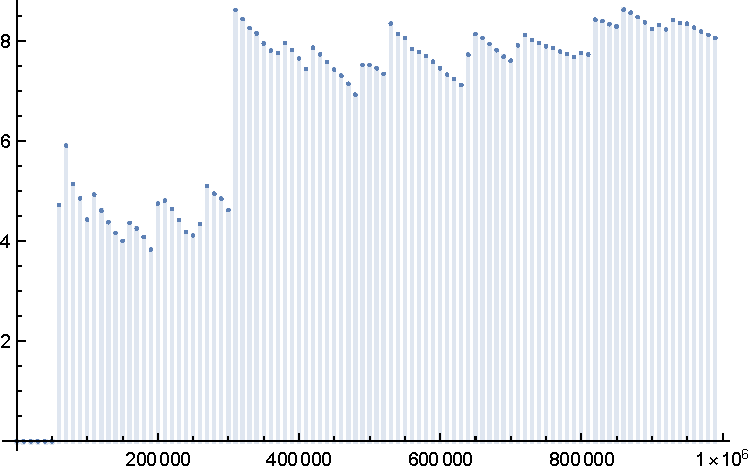
\includegraphics[width=0.8\textwidth]{abbildungen/auswertung1500/meanQueueTimePlot.pdf}
	\caption{Mittlere Warteschlangenlänge, MeanAr = 1500}
	\label{fig:meanQueueTime1500}
\end{figure}

\begin{figure}[htpb]
	\centering
	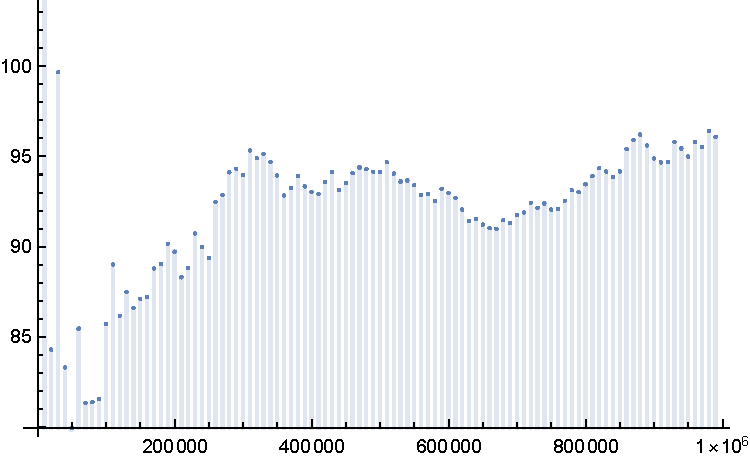
\includegraphics[width=0.8\textwidth]{abbildungen/auswertung1500/meanCallingTimePlot.pdf}
	\caption{Mittlere Telefonierdauer, MeanAr = 1500}
	\label{fig:meanCallingTime1500}
\end{figure}

\begin{figure}[htpb]
	\centering
	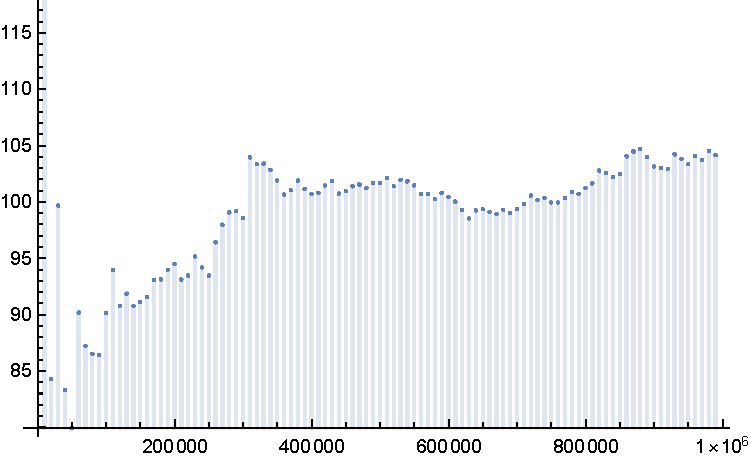
\includegraphics[width=0.8\textwidth]{abbildungen/auswertung1500/meanSystemTimePlot.pdf}
	\caption{Mittlere Zeit im System (Wartezeit + Telefonierdauer), MeanAr = 1500}
	\label{fig:meanSystemTime1500}
\end{figure}
\paragraph{Simulation und Berechnung in Java}


\subsubsection{Durchschnittliche Ankunftszeit der Clients: 1000}
\paragraph{Verwendung der Mathematica Simulation}
- Bild der Simulation 
- Plot Little-Law
- MeanSystemSize, MeanSystemTime, MeanQueueSize,MeanQueueTime aufführen
\paragraph{Verwendung der implementierten Java-Simulation, Berechnung in Mathematica}
\begin{figure}[htpb]
	\centering
	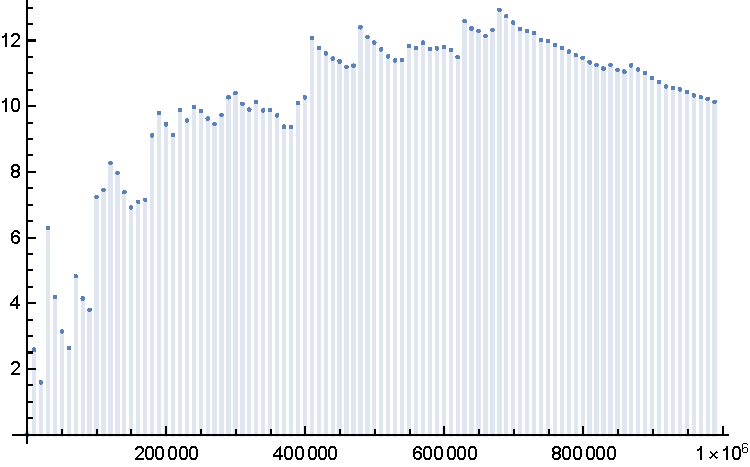
\includegraphics[width=0.8\textwidth]{abbildungen/auswertung1000/meanQueueTimePlot.pdf}
	\caption{Mittlere Warteschlangenlänge, MeanAr = 1000}
	\label{fig:meanQueueTime1000}
\end{figure}

\begin{figure}[htpb]
	\centering
	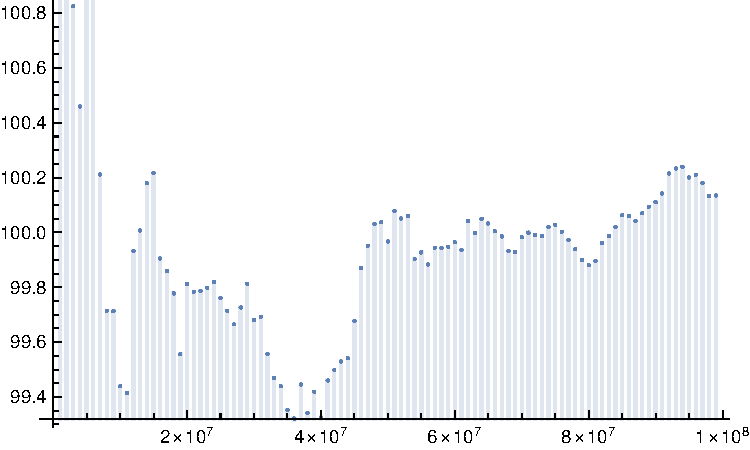
\includegraphics[width=0.8\textwidth]{abbildungen/auswertung1000/meanCallingTimePlot.pdf}
	\caption{Mittlere Telefonierdauer, MeanAr = 1000}
	\label{fig:meanCallingTime1000}
\end{figure}

\begin{figure}[htpb]
	\centering
	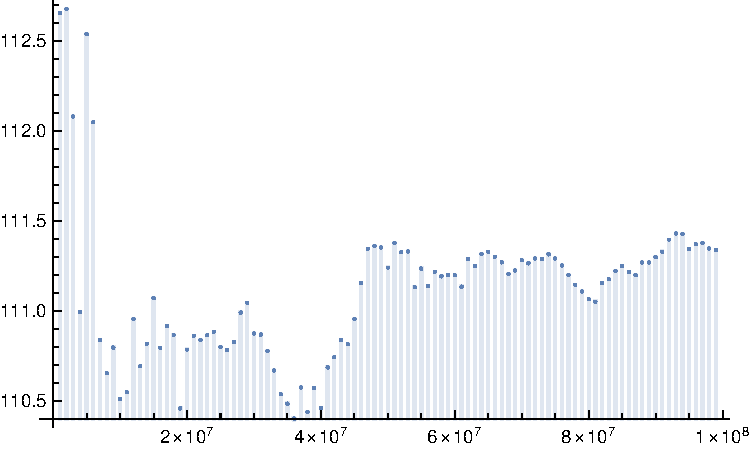
\includegraphics[width=0.8\textwidth]{abbildungen/auswertung1000/meanSystemTimePlot.pdf}
	\caption{Mittlere Zeit im System (Wartezeit + Telefonierdauer), MeanAr = 1000}
	\label{fig:meanSystemTime1000}
\end{figure}

\paragraph{Simulation und Berechnung in Java}


\subsubsection{Durchschnittliche Ankunftszeit der Clients: 500}
\paragraph{Verwendung der Mathematica Simulation}
- Bild der Simulation 
- Plot Little-Law
- MeanSystemSize, MeanSystemTime, MeanQueueSize,MeanQueueTime aufführen
\paragraph{Verwendung der implementierten Java-Simulation, Berechnung in Mathematica}
\begin{figure}[htpb]
	\centering
	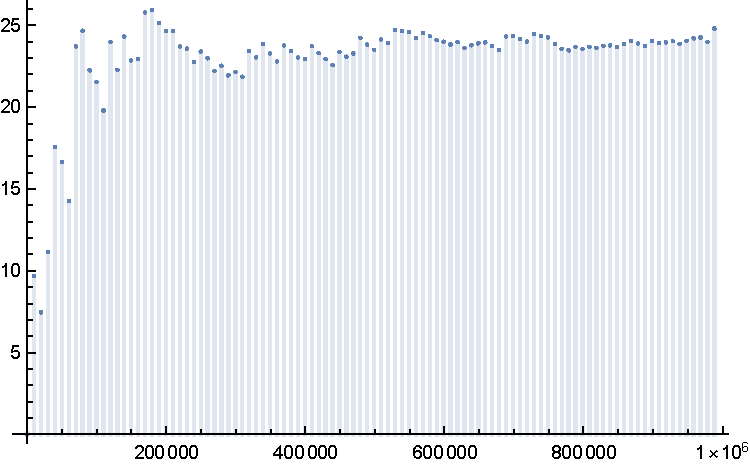
\includegraphics[width=0.8\textwidth]{abbildungen/auswertung500/meanQueueTimePlot.pdf}
	\caption{Mittlere Warteschlangenlänge, MeanAr = 500}
	\label{fig:meanQueueTime500}
\end{figure}

\begin{figure}[htpb]
	\centering
	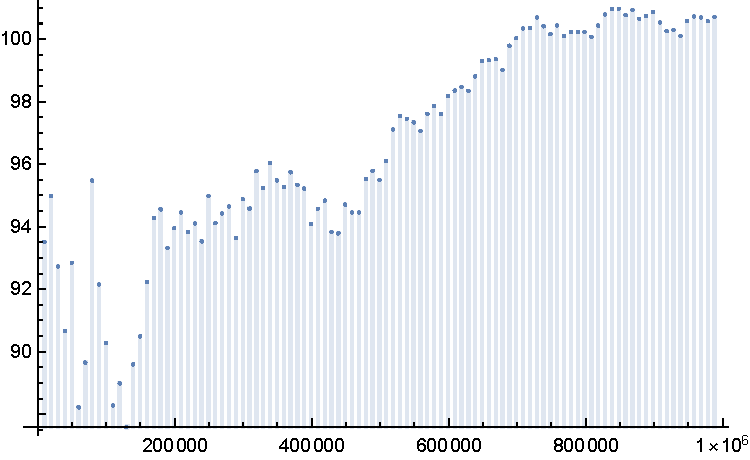
\includegraphics[width=0.8\textwidth]{abbildungen/auswertung500/meanCallingTimePlot.pdf}
	\caption{Mittlere Telefonierdauer, MeanAr = 500}
	\label{fig:meanCallingTime500}
\end{figure}

\begin{figure}[htpb]
	\centering
	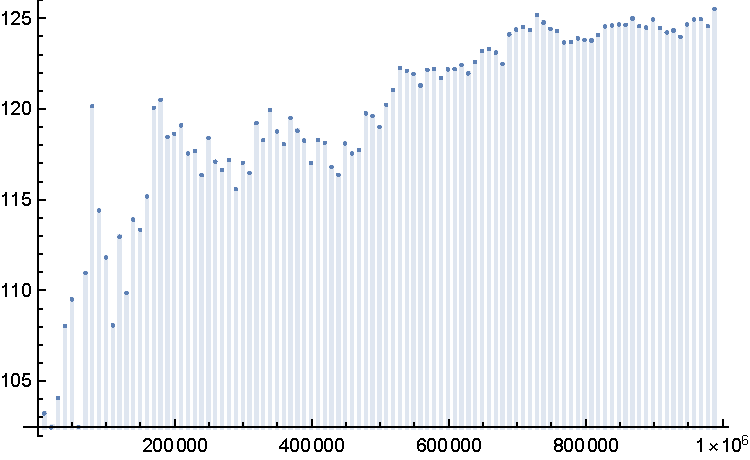
\includegraphics[width=0.8\textwidth]{abbildungen/auswertung500/meanSystemTimePlot.pdf}
	\caption{Mittlere Zeit im System (Wartezeit + Telefonierdauer), MeanAr = 500}
	\label{fig:meanSystemTime500}
\end{figure}
\paragraph{Simulation und Berechnung in Java}


\subsubsection{Durchschnittliche Ankunftszeit der Clients: 100}
\paragraph{Verwendung der Mathematica Simulation}
- Bild der Simulation 
- Plot Little-Law
- MeanSystemSize, MeanSystemTime, MeanQueueSize,MeanQueueTime aufführen

\paragraph{Verwendung der implementierten Java-Simulation, Berechnung in Mathematica}
Die berechneten Werte sind im folgenden aufgeführt:
\[\begin{array}{cc}
 \text{mean queue size} & 0.00537307572764891636692565082375430880024384373 \\
 \text{mean queue time} & 8.19291 \\
 \text{mean system size} & 0.06921258430823697932263116253494454280311475015 \\
 \text{mean system time} & 105.458 \\
\end{array}\]


\begin{figure}[htpb]
	\centering
	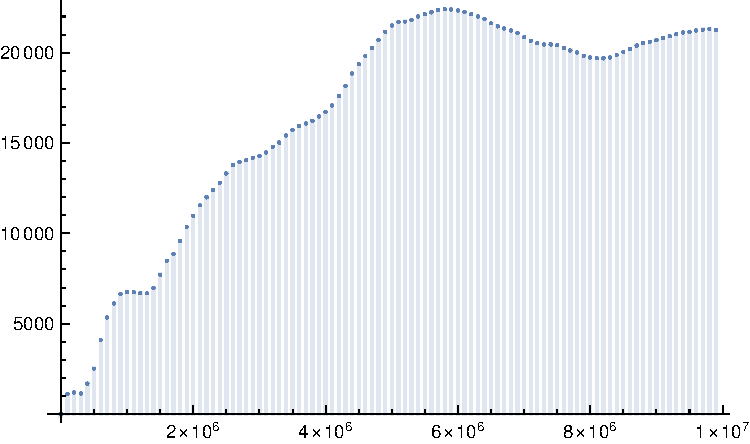
\includegraphics[width=0.8\textwidth]{abbildungen/auswertung100/meanQueueTimePlot.pdf}
	\caption{Mittlere Warteschlangenlänge, MeanAr = 100}
	\label{fig:meanQueueTime100}
\end{figure}
Betrachtet man die in \ref{fig:meanQueueTime100} abgebildete mittlere Warteschlangenlänge, fällt auf, dass sich diese bei ca. 11,1 einpendelt. Ab einer Simulationsdauer von $4*10^7$ ändert sich der Wert nur noch minimal. Dies deutet auf den sog. \glqq Steady State\grqq, den eingeschwungenen Zustand hin.

\begin{figure}[htpb]
	\centering
	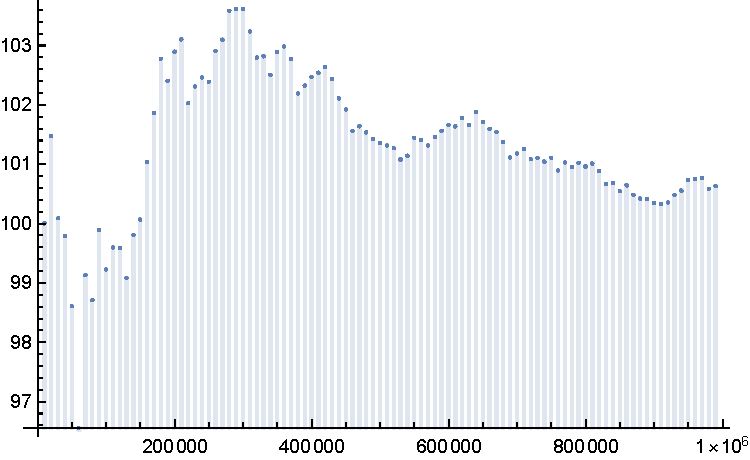
\includegraphics[width=0.8\textwidth]{abbildungen/auswertung100/meanCallingTimePlot.pdf}
	\caption{Mittlere Telefonierdauer, MeanAr = 100}
	\label{fig:meanCallingTime100}
\end{figure}

Abbildung \ref{fig:meanCallingTime100} zeigt die Änderung der mittleren Telefonierdauer über die Zeit. Wie auch in Abbildung \ref{fig:meanQueueTime100} werden die Sprünge zwischen den einzelnen Werten erwartungsgemäß immer geringer mit fortschreitender Simulationsdauer. Allerdings weißt die mittlere Telefonierdauer bis zum Ende der Simulation noch kleinere Wertänderungen auf. Wenn überhaupt, kann, basieren auf diesem Wert, erst ab einer Simulationsdauer von ca. $8*10^7$ von einem eingeschwungenen System ausgegangen werden.

\begin{figure}[htpb]
	\centering
	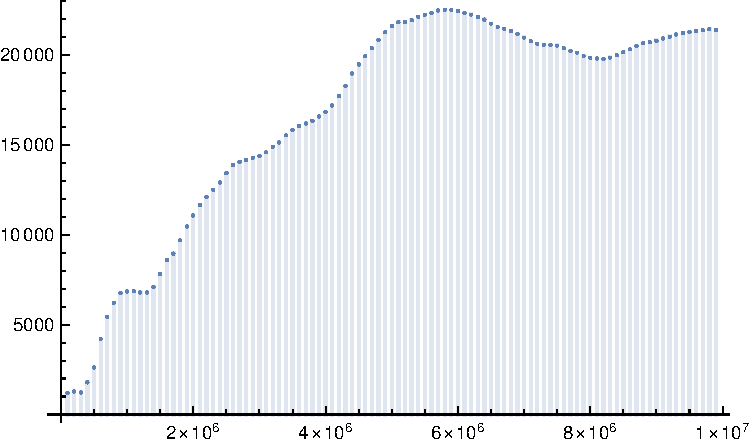
\includegraphics[width=0.8\textwidth]{abbildungen/auswertung100/meanSystemTimePlot.pdf}
	\caption{Mittlere Zeit im System (Wartezeit + Telefonierdauer), MeanAr = 100}
	\label{fig:meanSystemTime100}
\end{figure}

Im Vergleich dazu zeigt \ref{fig:meanSystemTime100} die durchschnittliche Zeit eines Clients im System. Diese berechnet sich durch die Summe aus durchschnittlicher Wartezeit und durchschnittlicher Telefonierdauer. Die Schwankungen zwischen den einzelnen Werten sind auf die erläuterten Wertänderungen bei der durchschnittlichen Telefonierdauer zurückzuführen. Gegen Ende der Simulation pendelt sich die durchschnittliche Systemzeit bei ca. $111,1$ ein.
  
\paragraph{Simulation und Berechnung in Java}




\subsection{Modell \glqq Bevorzugte VIP\grqq} 
\subsubsection{Durchschnittliche Ankunftszeit der Clients: 100}
\subsubsection{Durchschnittliche Ankunftszeit der Clients: 500}
\subsubsection{Durchschnittliche Ankunftszeit der Clients: 1000}
\subsubsection{Durchschnittliche Ankunftszeit der Clients: 1500}

\subsection{Modell \glqq Zusätzliches VIP Telefon\grqq} 
\subsubsection{Durchschnittliche Ankunftszeit der Clients: 100}
\subsubsection{Durchschnittliche Ankunftszeit der Clients: 500}
\subsubsection{Durchschnittliche Ankunftszeit der Clients: 1000}
\subsubsection{Durchschnittliche Ankunftszeit der Clients: 1500}

\section{Fazit}

\end{document}
